%!TEX root =  ssmr_ieee.tex

\section{Background and motivation}
%\section{State-machine replication}
\label{sec:smr}

State-machine replication is a fundamental approach to implementing a fault-tolerant service by replicating servers and coordinating the execution of client commands against server replicas~\cite{Lam78, Sch90}. 
The service is defined by a state machine, which consists of a set of \emph{state variables} $\vvm = \{v_1, ..., v_m\}$ 
%that encode the service's state 
and a set of \emph{commands} that may read and modify state variables, and produce a response for the command.
Each command is implemented by a deterministic program.
% whose execution is atomic with respect to other commands.
%The set of variables read by $C$ and the set of variables updated by $C$ are denoted, respectively, by $readset(C)$ and $writeset(C)$.
%The set of all variables read and updated by $C$ is denoted by $var(C)$. 
State-machine replication can be implemented with atomic broadcast: commands are atomically broadcast to all servers, and all correct servers deliver and execute the same sequence of commands.

We are interested in implementations of state-machine replication that ensure linearizability.
%
Linearizability is defined with respect to a sequential specification.
The \emph{sequential specification} of a service consists of a set of commands and a set of \emph{legal sequences of commands}, which define the behavior of the service when it is accessed sequentially.
In a legal sequence of commands, every response to the invocation of a command immediately follows its invocation, with no other invocation or response in between them.
For example, a sequence of operations for a read-write variable $v$ is legal if every read command returns the value of the most recent write command that precedes the read, if there is one, or the initial value otherwise.
An execution \ex\ is linearizable if there is some permutation of the commands executed in \ex\ that respects (i)~the service's sequential specification and (ii)~the real-time precedence of commands.
Command $C_1$ precedes command $C_2$ if the response of $C_1$ occurs before the invocation of $C_2$.

%The precise way in which the technique is implemented
%depends on the targeted consistency criterion, which in this paper we assume to be \emph{linearizability}. Once we prove that S-SMR provides such level of consistency, performance-optimized variations of S-SMR can be achieved later on by relaxing such consistency requirement. We can define linearizability intuitively: an execution in a replicated system is linearizable if the application program that uses such system gets the same behavior as with a single site, unreplicated system; hence, writing the application logic is no different to conventional programming~\cite{replication2010pedone}.

%To define linearizability more formally, we need the notion of \emph{sequential specification} for the variables, which determines whether a sequence of commands (and their matching responses) is legal, given a set of variables \mbox{$\vvm = \{v_1, ..., v_m\}$} stored in the servers. For example, the sequential specification for read-write variables is: given a sequence $\sigma$ of commands, the response given to any command $x$ that reads some variable $v$ must be coherent with the most recent command that writes $v$ and precedes $x$ in $\sigma$. Also, we need the notion of \emph{real-time precedence}, denoted by $<_{RT}$. We say that commands $x$ and $y$ are such that $x <_{RT} y$ if the response to command $x$ is received before command $y$ is issued, in real-time. Finally, execution \ex\ is linearizable if there is some permutation $\pi$ of the commands executed in \ex\, such that (i)~the sequential specification of every variable is respected in $\pi$ and (ii)~if $x <_{RT} y$, then $x$ precedes $y$ in $\pi$~\cite{Attiya04}.

%The execution in Fig.~\ref{fig:linvsnonlin} (top) is not linearizable because the reordering of commands that form a legal sequence (i.e., $C_1$, $C_3$, $C_2$) does not respect the real-time precedence of commands (i.e., it violates the real-time ordering of $C_2$ and $C_3$).
%%: we can see that $C_1 <_{RT} C_2 <_{RT} C_3$, but a permutation that respected such real-time precedence would not be legal. 
%In Fig.~\ref{fig:linvsnonlin} (bottom), however, there is no real-time precedence between $C_2$ and $C_3$, because $C_3$ was issued by client $b$ before client $a$ received the reply for $C_2$. For this reason, the execution is linearizable.
%
%\begin{figure}[ht]
%  \begin{center}
%    \begin{tabular}{c}
%      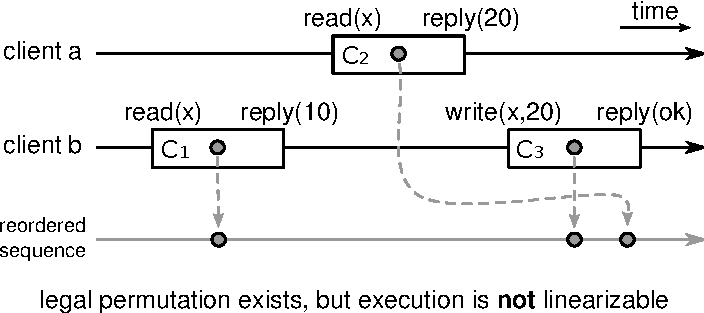
\includegraphics[width=0.9\columnwidth]{figures/nonlinearizable} \\
%      \\
%      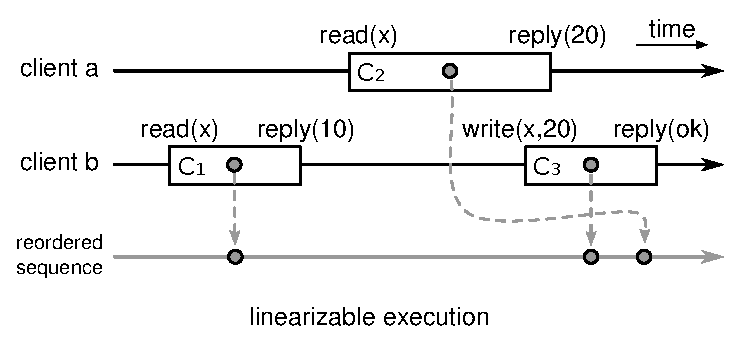
\includegraphics[width=0.9\columnwidth]{figures/linearizable} \\
%    \end{tabular}
%    \caption{Linearizable vs. non-linearizable executions.}
%    \label{fig:linvsnonlin}
%  \end{center}
%% \vspace{-4mm}
%\end{figure}


%State-machine replication implements linearizability by regulating how client commands are propagated to and executed by the replicas: 
%(i)~every nonfaulty replica must receive every command;  and
%(ii)~replicas must agree on the order of received and executed commands.
%Since each command is implemented by a deterministic program, each replica will produce the same state changes and response upon executing the same sequence of commands.
%State-machine replication can be implemented with atomic broadcast: commands are atomically broadcast to all servers, and all correct servers deliver and execute the same sequence of commands.
%%Since execution is deterministic, every server reaches the same state and produces the same response after executing a  command.

%\subsection{On the (lack of) scalability of SMR}

In classical state-machine replication, throughput does not scale with the number of replicas: each command must be ordered among replicas and executed and replied by every (non-faulty) replica.
Some simple optimizations to the traditional scheme can provide improved performance but not scalability.
For example, although update commands must be ordered and executed by every replica, only one replica can respond to the client, saving resources at the other replicas.
Commands that only read the state must be ordered with respect to other commands, but can be executed by a single replica, the replica that will respond to the client.

%A simple analysis shows that these schemes do not scale with the number of servers.
%Assume a replica needs $\delta_o$ time units to order a command, $\delta_e$ time units to execute the command, and $\delta_r$ time units to respond to the client---for simplicity, we consider $\delta_o$ to be constant with the number of servers.
%%~\cite{Marandi10}.
%In this model, traditional state-machine replication has throughput of $1/(\delta_o+\delta_e+\delta_r)$.
%The optimizations for update and read-only commands improve throughput to $N/(\delta_o+\delta_e+\delta_r/N)$ and $N/(\delta_o+(\delta_e+\delta_r)/N)$, respectively, where $N$ is the number of replicas.
%A scalable system would have throughput that grows proportionally with the number of servers.
%Figure~\ref{fig:scale} compares the behavior of traditional state-machine replication and the update and read-only optimizations with a truly scalable implementation. In the figure, we assume $\delta_o=\delta_e=\delta_r$; different values of $\delta$ would not change the asymptotic behavior of the techniques.
%
%
%\begin{figure}[ht]
%  \begin{center}
%      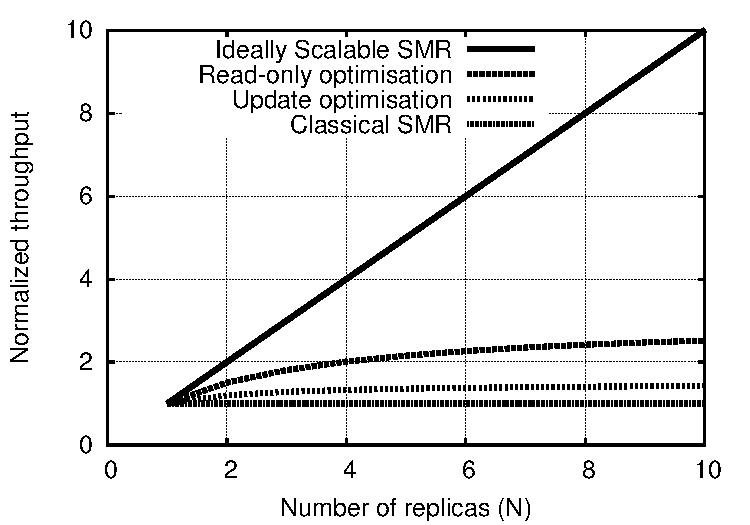
\includegraphics[width=0.9\columnwidth]{graphs/smr-scal/scale.pdf} 
%    \caption{Scalability of SMR implementations.}
%        \label{fig:scale}
%  \end{center}
%\end{figure}


%Such traditional implementations of SMR, however, has limited scalability. Adding servers to the system may not increase its throughput, and is likely, instead, to create a larger overhead on the group-communication component of the system, responsible for implementing atomic multicast. Note that servers can divide the execution of read-only commands (only one server has to execute, since no state is changed) and the sending of replies to write commands (although the state must change in all servers, one reply is enough). In the best case, i.e., in a workload dominated by read-only commands, this would approximate a linear increase of throughput, relatively to the number of servers. However, the group communication component of the system would have to increase its capacity as well, in order to avoid becoming a bottleneck, but its cost, in number of internal messages, would grow linearly (at least) to the number of processes in such component,\footnote{To the best of our knowledge, Ring-Paxos~\cite{Marandi10} requires the lowest number of messages for a consensus algorithm, which is $O(a)$, where $a$ is the number of acceptors.} eventually weighing out the linear (at best) throughput gain. In any case, even with a read-only workload, every server would have to deliver every single command, which alone would prevent the system from scaling.

This is a fundamental limitation: while some optimizations may increase throughput by adding servers, the improvements are limited since fundamentally, the technique does not scale.
In the next section, we describe an extension to SMR that under certain workloads allows performance to grow proportionally to the number of replicas.


%State-machine replication can be implemented with atomic multicast: if all servers belong to the same group and all commands are atomically multicast to such group, then all correct servers deliver and execute the same sequence of commands, i.e., they execute the commands in the same order. Moreover, if all servers have each a full copy of the application state, they all start at the same initial state, and command execution is deterministic, then every server reaches the same state after executing a given command and, thus, no two servers give different responses to the same command.



%\clearpage